\documentclass{standalone}
\usepackage{pgf, tikz}
\usetikzlibrary{arrows, automata, positioning}

\begin{document}

    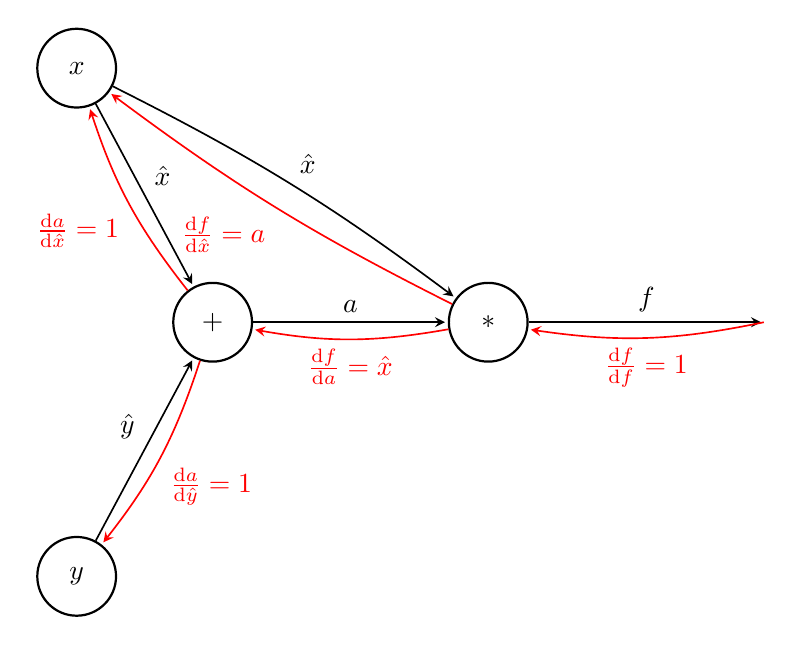
\begin{tikzpicture}[
            > = stealth, 
            shorten > = 1pt, 
            auto,
            node distance = 3.5cm,
            semithick
        ]

        \tikzstyle{every state}=[
            draw = black,
            thick,
            fill = white,
            minimum size = 10mm
        ]
        %\tikzset{every edge/.append style={font=\large}}

		\node[state] (add) {$+$};
        \node[state] (x) [above left=2.5cm and 1cm of add] {$x$};
        \node[state] (y) [below left=2.5cm and 1cm of add] {$y$};        
        \node[state] (mul) [right of=add] {$*$};
        \coordinate[right of=mul] (f);
        
        \path[->] (x) edge node {$\hat{x}$} (add);        
        \path[->] (x) edge [bend left=5] node {$\hat{x}$} (mul);        
        \path[->] (y) edge node {$\hat{y}$} (add);        
        \path[->] (add) edge node {$a$} (mul);
        \path[->] (mul) edge node {$f$} (f);
      
        % partial edges
        \iftrue
        \path[->] (add) edge [red, bend left=10] node {$\frac{\mathrm{d}a}{\mathrm{d}\hat{x}} = 1$} (x);
        \path[->] (mul) edge [red, bend left=5] node {$\frac{\mathrm{d}f}{\mathrm{d}\hat{x}} = a$} (x);
        \path[->] (add) edge [red, bend left=10] node {$\frac{\mathrm{d}a}{\mathrm{d}\hat{y}} = 1$} (y);
        \path[->] (mul) edge [red, bend left=10] node {$\frac{\mathrm{d}f}{\mathrm{d}a} = \hat{x}$} (add);
        \path[->] (f) edge [red, bend left=10] node {$\frac{\mathrm{d}f}{\mathrm{d}f} = 1$} (mul);
        \fi
        

    \end{tikzpicture}

\end{document}